
\section{Limites et motivation}

\begin{frame}{Du mur de la scalabilité à l’approche par collisions}

    \begin{block}{Explosion combinatoire (Speck 32/64, 3 tours, $p = 2^{-3}$)}
        \centering
        \renewcommand{\arraystretch}{1.2}
        \small
        \begin{tabular}{lcc}
            \toprule
            \textbf{Algorithme} & \textbf{Complexité} & \textbf{Faisabilité} \\
            \midrule
            Naïf exhaustif & $\mathcal{O}(2^{2n})$ & Abandonné \\
            Naïf optimisé  & $\mathcal{O}(2^n \cdot p^{-1})$ & Limite pratique \\
            Collisions & $\mathcal{O}(2^{n/2} \cdot p^{-1})$ & Réalisable \\
            \bottomrule
        \end{tabular}
    \end{block}

    \vspace{0.2cm}

    \begin{itemize}\small
        \item Explosion combinatoire dès $n=32$ : approche exhaustive inutilisable.
        \item Même optimisée, la recherche reste coûteuse (ordre de $10^4$ s).
        \item Nécessité de changer de paradigme algorithmique.
    \end{itemize}

    \vspace{0.2cm}

    \begin{block}{Idée clé}
        Remplacer la recherche exhaustive de $\alpha$ par la détection de \textbf{collisions sur une fonction dérivée}.
    \end{block}

\end{frame}

% =========================================================
% SQUELETTE SLIDE 2
% =========================================================
% --- DIAPO 2 : VALIDATION SPECK 32/64 ---
\section{Validation expérimentale}

\begin{frame}{Validation expérimentale sur Speck 32/64}

    \begin{block}{Objectif expérimental}
        Vérifier la validité des résultats théoriques sur Speck 32/64 en conditions réelles de calcul.
    \end{block}

    \vspace{0.2cm}

    \begin{itemize}\small
        \item Cible : Speck 32/64 sur des caractéristiques issues des résultats théoriques.
        \item Approche : exécution sur un ensemble de clés aléatoires.
        \item Mesure : estimation empirique des probabilités différentielles.
    \end{itemize}

    \vspace{0.2cm}

    \begin{block}{Contraintes expérimentales}
        \begin{itemize}\small
            \item Limitation mémoire : segmentation en lots de calcul.
            \item Limitation temps : compromis temps/mémoire nécessaire.
            \item Fort coût de calcul dès $p \leq 2^{-9}$.
        \end{itemize}
    \end{block}

    \vspace{0.2cm}

\end{frame}

% =========================================================
% SQUELETTE SLIDE 3
% =========================================================
% --- DIAPO : DIAGRAMME DES CLÉS (ÉPURÉE) ---
\begin{frame}{Distribution des probabilités sur les clés (Speck 32/64, 5 tours)}

    \begin{block}{Configuration}
        \small 1000 clés testées \quad ($p \approx 2^{-9}$)
    \end{block}

    \vspace{0.2cm}

    \begin{center}
        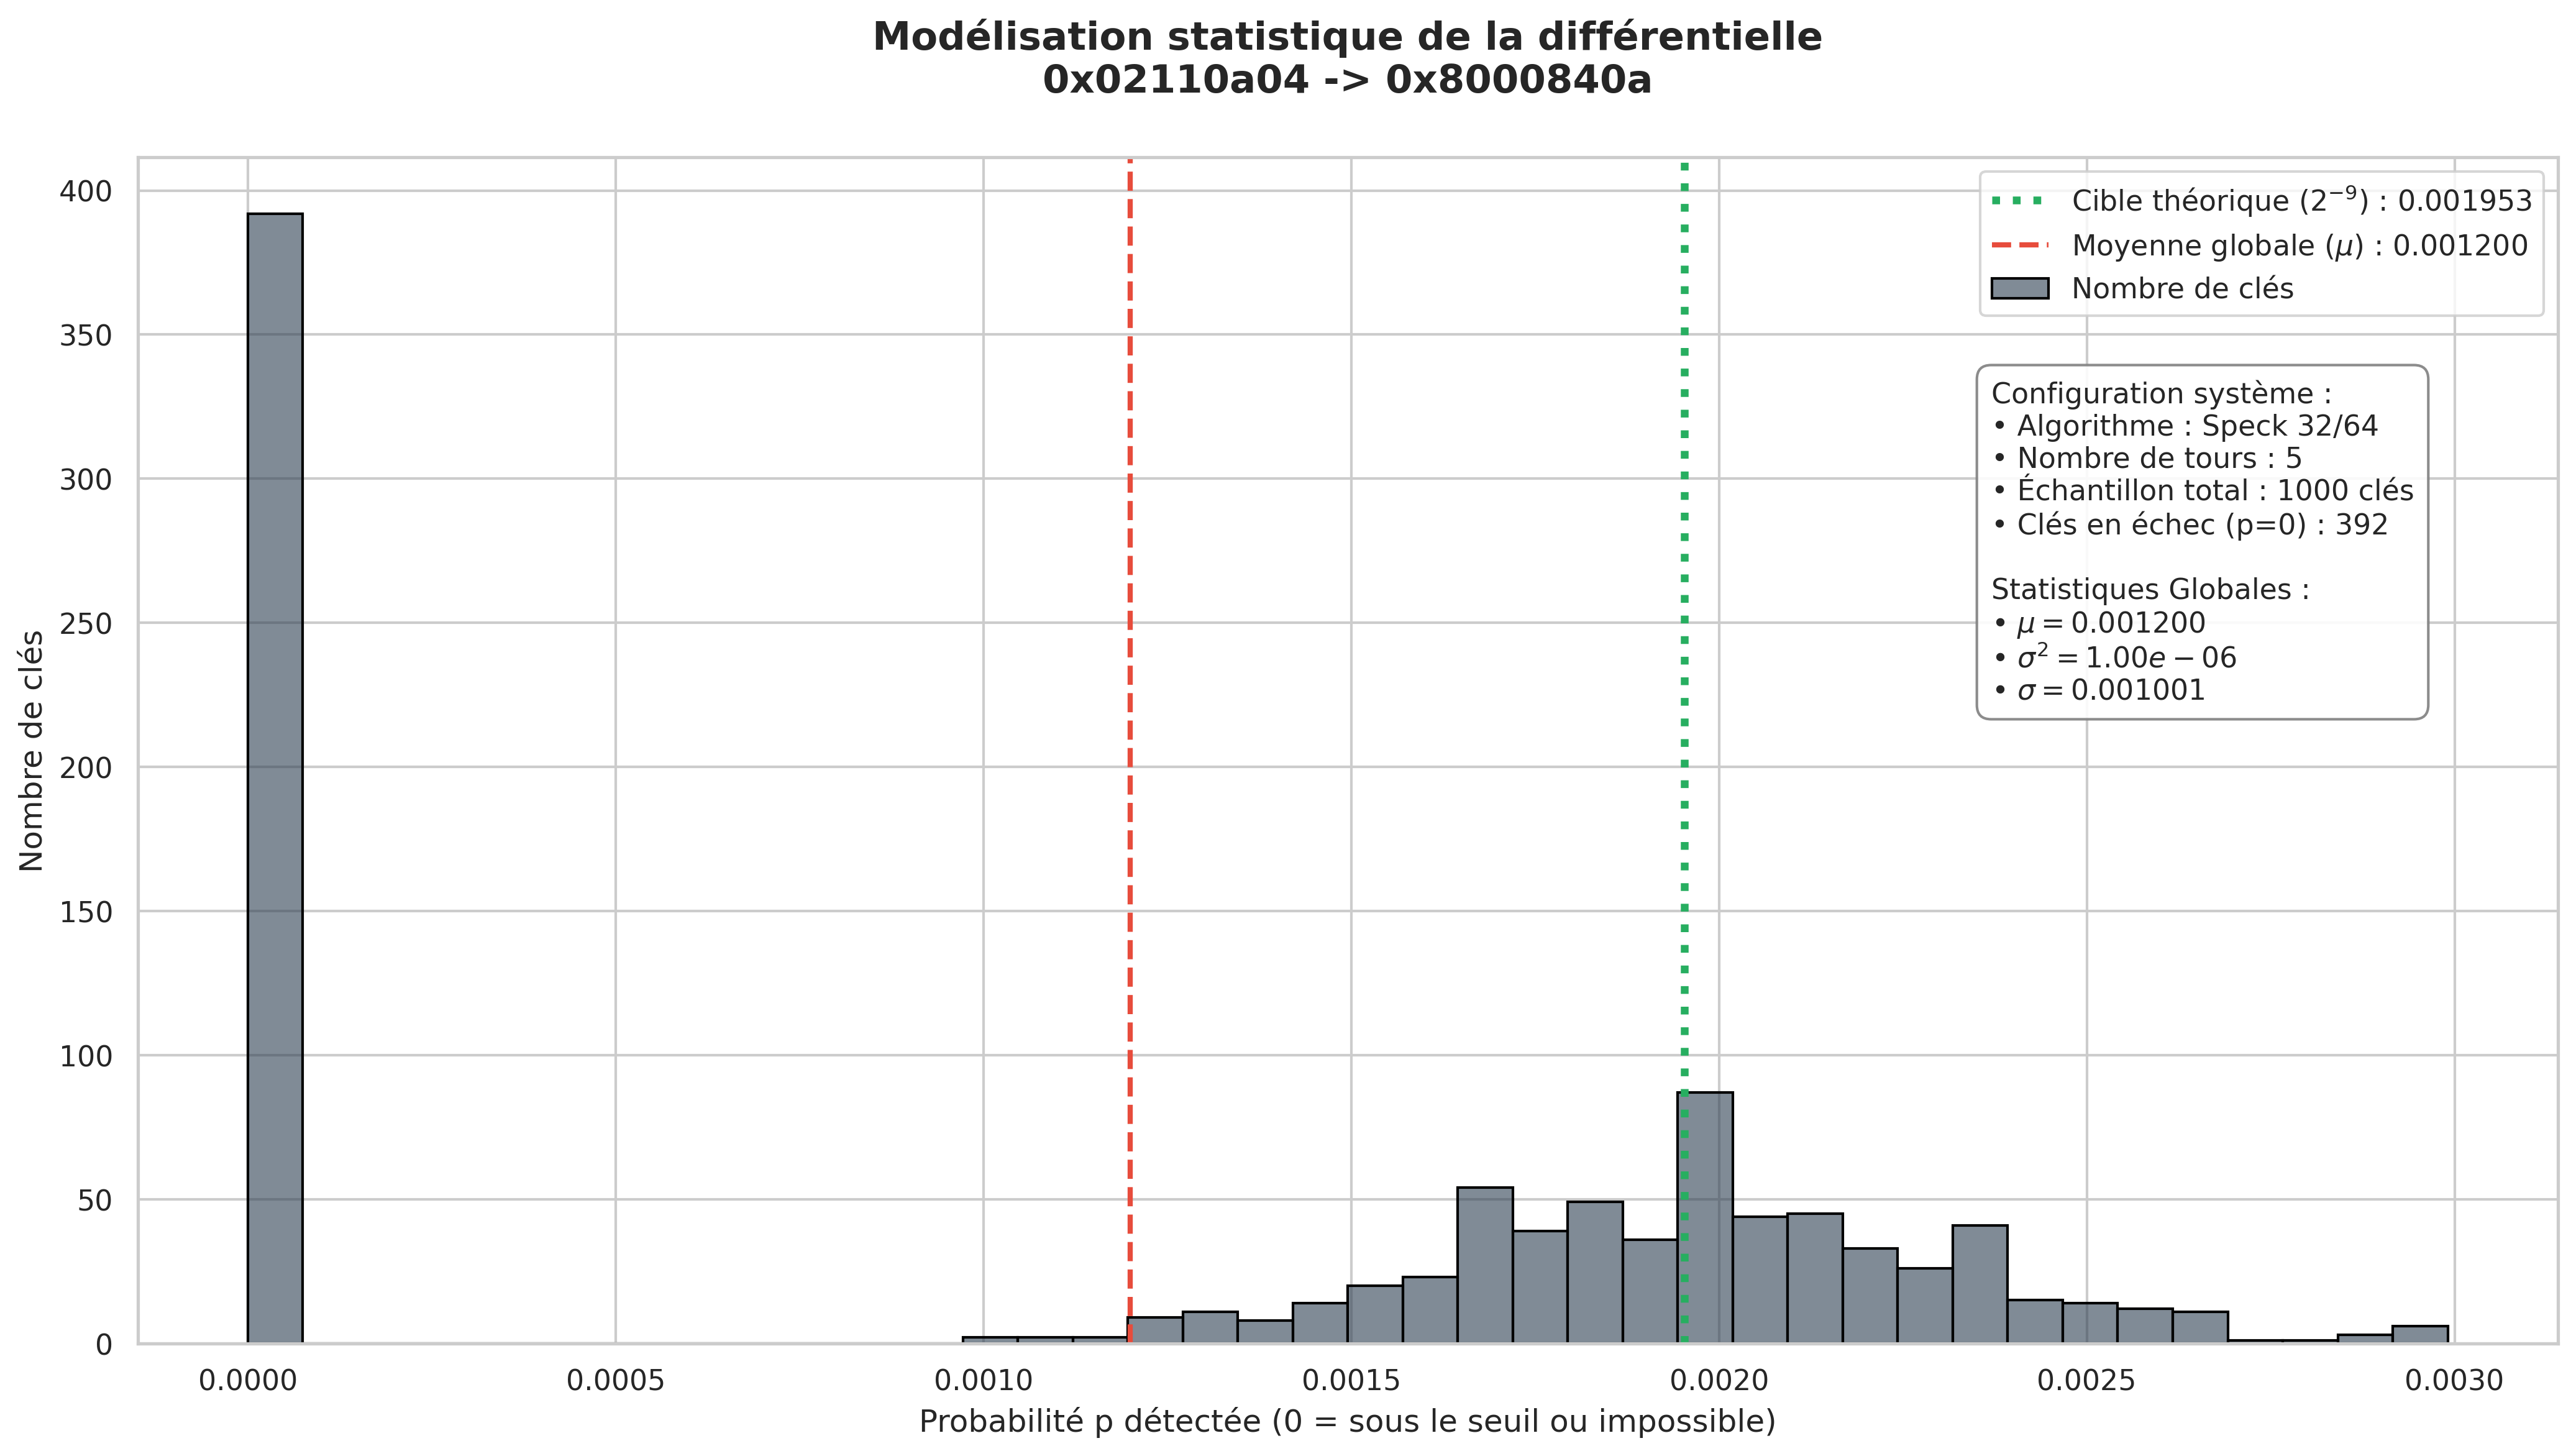
\includegraphics[width=0.8\textwidth,height=0.5\textheight,keepaspectratio]{figures/analyse_globale_speck_5tours.png}
    \end{center}

\end{frame}
% =========================================================
% SQUELETTE SLIDE 4
% =========================================================
% --- DIAPO : POURQUOI LES CLÉS NE SONT PAS DÉTECTÉES ---
\begin{frame}{Pourquoi certaines clés ne sont pas détectées ?}

    \begin{block}{Observation}
        Une proportion importante de clés ($\sim$ 40\%) ne produit aucune collision détectable.
    \end{block}

    \vspace{0.3cm}

    \begin{itemize}\small
        \item \textbf{Échantillonnage limité :} peu de substituts $\gamma$ testés (batching).
        \item \textbf{Hypothèse imparfaite :} $g_\gamma$ n’est pas parfaitement aléatoire.
        \item \textbf{Effet clé-dépendant :} certaines clés “s’accordent mal” avec les $\gamma$ choisis.
    \end{itemize}

    \vspace{0.3cm}

    \begin{block}{Conséquence}
        Absence de collision $\;\Rightarrow\;$ la différentielle existe, mais reste \textbf{invisible} pour l’algorithme.
    \end{block}

\end{frame}

% =========================================================
% SQUELETTE SLIDE 5
% =========================================================
% --- DIAPO : SPECK 6 TOURS ---
\begin{frame}{Speck 32/64 (6 tours) : résultats expérimentaux}

    \begin{block}{Contexte}
        \small Probabilité faible ($p \approx 2^{-13}$) $\Rightarrow$ utilisation d’un \textbf{compromis Temps/Mémoire (Tradeoff)}
    \end{block}

    \vspace{0.2cm}

    \centering
    \renewcommand{\arraystretch}{1.2}
    \scriptsize
    \begin{tabular}{lll}
        \toprule
        \textbf{$\alpha$} & \textbf{$\beta$} & \textbf{Probabilité} \\
        \midrule
        \texttt{0x02110a04} & \texttt{0x8d0a9d20} & 0,000145 \\
        \textbf{\texttt{0x02110a04}} & \textbf{\texttt{0x850a9520}} & \textbf{0,000092} \\
        \texttt{0x020f0a04} & \texttt{0x850a9520} & 0,000084 \\
        \texttt{0x02110a04} & \texttt{0x851a9530} & 0,000076 \\
        \texttt{0x02110a04} & \texttt{0x8f0a9f20} & 0,000076 \\
        \texttt{0x02110a04} & \texttt{0x830a9320} & 0,000072 \\
        \bottomrule
    \end{tabular}

    \vspace{0.2cm}

    \begin{itemize}\small
        \item Le meilleur candidat mesuré n’est pas celui attendu.
        \item \textbf{Biais d’échantillonnage} : estimation locale trompeuse.
        \item Vérification globale $\Rightarrow$ confirmation du résultat théorique ($\approx 2^{-13}$).
    \end{itemize}

\end{frame}

% =========================================================
% SQUELETTE SLIDE 6
% =========================================================
\begin{frame}{Résultats (6 tours Speck)}
    % TODO tableau 6 tours
\end{frame}

% =========================================================
% SQUELETTE SLIDE 7
% =========================================================
\begin{frame}{Conclusion / limites}
    \begin{itemize}
        \item Synthèse
        \item Limites mémoire
        \item Perspectives GPU
    \end{itemize}
\end{frame}

\end{document}
